% $Id: template.tex 11 2007-04-03 22:25:53Z jpeltier $

\documentclass{vgtc}                          % final (conference style)
%\documentclass[review]{vgtc}                 % review
%\documentclass[widereview]{vgtc}             % wide-spaced review
%\documentclass[preprint]{vgtc}               % preprint
%\documentclass[electronic]{vgtc}             % electronic version

%% Uncomment one of the lines above depending on where your paper is
%% in the conference process. ``review'' and ``widereview'' are for review
%% submission, ``preprint'' is for pre-publication, and the final version
%% doesn't use a specific qualifier. Further, ``electronic'' includes
%% hyperreferences for more convenient online viewing.

%% Please use one of the ``review'' options in combination with the
%% assigned online id (see below) ONLY if your paper uses a double blind
%% review process. Some conferences, like IEEE Vis and InfoVis, have NOT
%% in the past.

%% Figures should be in CMYK or Grey scale format, otherwise, colour 
%% shifting may occur during the printing process.

%% These few lines make a distinction between latex and pdflatex calls and they
%% bring in essential packages for graphics and font handling.
%% Note that due to the \DeclareGraphicsExtensions{} call it is no longer necessary
%% to provide the the path and extension of a graphics file:
%% \includegraphics{diamondrule} is completely sufficient.
%%
\ifpdf%                                % if we use pdflatex
  \pdfoutput=1\relax                   % create PDFs from pdfLaTeX
  \pdfcompresslevel=9                  % PDF Compression
  \pdfoptionpdfminorversion=7          % create PDF 1.7
  \ExecuteOptions{pdftex}
  \usepackage{graphicx}                % allow us to embed graphics files
  \DeclareGraphicsExtensions{.pdf,.png,.jpg,.jpeg} % for pdflatex we expect .pdf, .png, or .jpg files
\else%                                 % else we use pure latex
  \ExecuteOptions{dvips}
  \usepackage{graphicx}                % allow us to embed graphics files
  \DeclareGraphicsExtensions{.eps}     % for pure latex we expect eps files
\fi%

%% it is recomended to use ``\autoref{sec:bla}'' instead of ``Fig.~\ref{sec:bla}''
\graphicspath{{figures/}{pictures/}{images/}{./}} % where to search for the images

\usepackage{microtype}                 % use micro-typography (slightly more compact, better to read)
\PassOptionsToPackage{warn}{textcomp}  % to address font issues with \textrightarrow
\usepackage{textcomp}                  % use better special symbols
\usepackage{mathptmx}                  % use matching math font
\usepackage{times}                     % we use Times as the main font
\renewcommand*\ttdefault{txtt}         % a nicer typewriter font
\usepackage{cite}                      % needed to automatically sort the references
\usepackage{tabu}                      % only used for the table example
\usepackage{booktabs}                  % only used for the table example
\usepackage{mdwlist}
\usepackage{coloremoji}
%% We encourage the use of mathptmx for consistent usage of times font
%% throughout the proceedings. However, if you encounter conflicts
%% with other math-related packages, you may want to disable it.


%% If you are submitting a paper to a conference for review with a double
%% blind reviewing process, please replace the value ``0'' below with your
%% OnlineID. Otherwise, you may safely leave it at ``0''.
\onlineid{0}

%% declare the category of your paper, only shown in review mode
\vgtccategory{Research}

%% allow for this line if you want the electronic option to work properly
\vgtcinsertpkg

%% In preprint mode you may define your own headline.
%\preprinttext{To appear in an IEEE VGTC sponsored conference.}

%% Paper title.

\title{Visualizing Low-Dimensional Word Embeddings with Emoji Annotators}

%% This is how authors are specified in the conference style

%% Author and Affiliation (single author).
%%\author{Roy G. Biv\thanks{e-mail: roy.g.biv@aol.com}}
%%\affiliation{\scriptsize Allied Widgets Research}

%% Author and Affiliation (multiple authors with single affiliations).
%%\author{Roy G. Biv\thanks{e-mail: roy.g.biv@aol.com} %
%%\and Ed Grimley\thanks{e-mail:ed.grimley@aol.com} %
%%\and Martha Stewart\thanks{e-mail:martha.stewart@marthastewart.com}}
%%\affiliation{\scriptsize Martha Stewart Enterprises \\ Microsoft Research}

%% Author and Affiliation (multiple authors with multiple affiliations)
%% Author and Affiliation (multiple authors with multiple affiliations)
\author{Yoshinari Fujinuma\thanks{e-mail: Yoshinari.Fujinuma@colorado.edu}\\ %
        \parbox{1.6in}{\scriptsize Department of Computer Science \\ University of Colorado Boulder} %
\and Shantanu Karnwal\thanks{e-mail: Shantanu.Karnwal@colorado.edu}\\ %
     \parbox{1.6in}{\scriptsize Department of Computer Science \\ University of Colorado Boulder}
     }

%% A teaser figure can be included as follows, but is not recommended since
%% the space is now taken up by a full width abstract.
%\teaser{
%  \includegraphics[width=1.5in]{sample.eps}
%  \caption{Lookit! Lookit!}
%}

%% Abstract section.
\abstract{Duis autem vel eum iriure dolor in hendrerit in vulputate
velit esse molestie consequat, vel illum dolore eu feugiat nulla
facilisis at vero eros et accumsan et iusto odio dignissim qui blandit
praesent luptatum zzril delenit augue duis dolore te feugait nulla
facilisi. Lorem ipsum dolor sit amet, consectetuer adipiscing elit,
sed diam nonummy nibh euismod tincidunt ut laoreet dolore magna
aliquam erat volutpat. Ut wisi enim ad minim veniam, quis nostrud exerci tation ullamcorper
suscipit lobortis nisl ut aliquip ex ea commodo consequat. Duis autem
vel eum iriure dolor in hendrerit in vulputate velit esse molestie
consequat, vel illum dolore eu feugiat nulla facilisis at vero eros et
accumsan et iusto odio dignissim qui blandit praesent luptatum zzril
delenit augue duis dolore te feugait nulla facilisi.%
} % end of abstract

%% ACM Computing Classification System (CCS). 
%% See <http://www.acm.org/about/class> for details.
%% We recommend the 2012 system <http://www.acm.org/about/class/class/2012>
%% For the 2012 system use the ``\CCScatTwelve'' which command takes four arguments.
%% The 1998 system <http://www.acm.org/about/class/class/2012> is still possible
%% For the 1998 system use the ``\CCScat'' which command takes four arguments.
%% In both cases the last two arguments (1998) or last three (2012) can be empty.

\CCScatlist{
  \CCScatTwelve{Human-centered computing}{Visu\-al\-iza\-tion}{Visu\-al\-iza\-tion techniques}{Treemaps};
  \CCScatTwelve{Human-centered computing}{Visu\-al\-iza\-tion}{Visualization design and evaluation methods}{}
}

%\CCScatlist{
  %\CCScat{H.5.2}{User Interfaces}{User Interfaces}{Graphical user interfaces (GUI)}{};
  %\CCScat{H.5.m}{Information Interfaces and Presentation}{Miscellaneous}{}{}
%}

%% Copyright space is enabled by default as required by guidelines.
%% It is disabled by the 'review' option or via the following command:
% \nocopyrightspace

%%%%%%%%%%%%%%%%%%%%%%%%%%%%%%%%%%%%%%%%%%%%%%%%%%%%%%%%%%%%%%%%
%%%%%%%%%%%%%%%%%%%%%% START OF THE PAPER %%%%%%%%%%%%%%%%%%%%%%
%%%%%%%%%%%%%%%%%%%%%%%%%%%%%%%%%%%%%%%%%%%%%%%%%%%%%%%%%%%%%%%%%

\begin{document}

%% The ``\maketitle'' command must be the first command after the
%% ``\begin{document}'' command. It prepares and prints the title block.

%% the only exception to this rule is the \firstsection command
\firstsection{Introduction}

\maketitle

%% \section{Introduction} %for journal use above \firstsection{..} instead
Word embeddings, especially cross-lingual embeddings, has been successful in multiple NLP applications such as machine translation \cite{lample2018unsupervised, artetxe2018unsupervised} and cross-lingual document classification \cite{klementiev-titov-bhattarai:2012:PAPERS}. 
But one area where there has not been very specific research is discovering the meanings of the embeddings themselves. \\

One way to efficiently convey this semantic information about embeddings is to enable an efficient interaction between humans and the visualizations of these embeddings. However, there have been a lot of problems in the current visualizations of these embeddings.
For example, there are potential problems of naively displaying the word embeddings projected onto 2D space using t-SNE \cite{t-sne}, which is not commonly used in visualizing word embeddings, such as;
\begin{itemize*}
  \item Overlap of words when zoomed out. 
  \item A counter-intuitive features of a t-SNE visualization (e.g., ``cluster sizes mean nothing''\footnote{https://distill.pub/2016/misread-tsne/}) 
  \item There are many other alternatives to visualize word embeddings than commonly used t-SNE (e.g., UMAP \cite{umap} or $k$-Nearest Neighbor graph), but no thorough comparison conducted. 
 %\item Which is the better way to display word embeddings to humans: k-nearest neighbor graph or t-SNE-based visualization? Does a counter-intuitive visualization using t-SNE \cite{t-sne} (e.g., ``cluster sizes mean nothing''\footnote{https://distill.pub/2016/misread-tsne/}) affect the interaction with humans? 
\end{itemize*}
Figure~\ref{fig:graph} shows an example of $k$-nearest neighbor graph and Figure~\ref{fig:t_sne} shows an example of visualization using t-SNE. \\

Also, many researchers decided to visualize embeddings in the 3D space, like Tensorboard \cite{tensorboard_viz}, but it ends up looking like a large cluttered collection of points. A visualization like that is just useful if the goal is to just play around with the click-and-drag interaction, but in the end, there is no semantic information being conveyed. \\

The ultimate goal of any good visualization is to convey the user about everything the data represents, and not what the data is like. Therefore, we think that semantics is a crucial aspect of any good visualization. So when we decided to carry on this project, the key question we asked ourselves was - How can we represent word embeddings efficiently in a 2D design space by keeping the clutter on the design space as minimum as possible? \\

Therefore using this motivation, we carry forward this project, and accomplished the following:
\begin{itemize*}
 \item Used a 2D design space to visualize the entire word2vec embedding space.
 \item Kept the clutter minimized by having an efficient k-means clustering algorithm implemented on the cosine similarities of these word vectors.
 \item Convey the semantic information of every single cluster by annotating them with Emojis, because of their excellent way of conveying semantic information with just a single character.
\end{itemize*}

\section{Description of the Project}
Figure~\ref{fig:cluster_network} shows the output of our visualization. 

\begin{figure}[htb]
 \centering
     {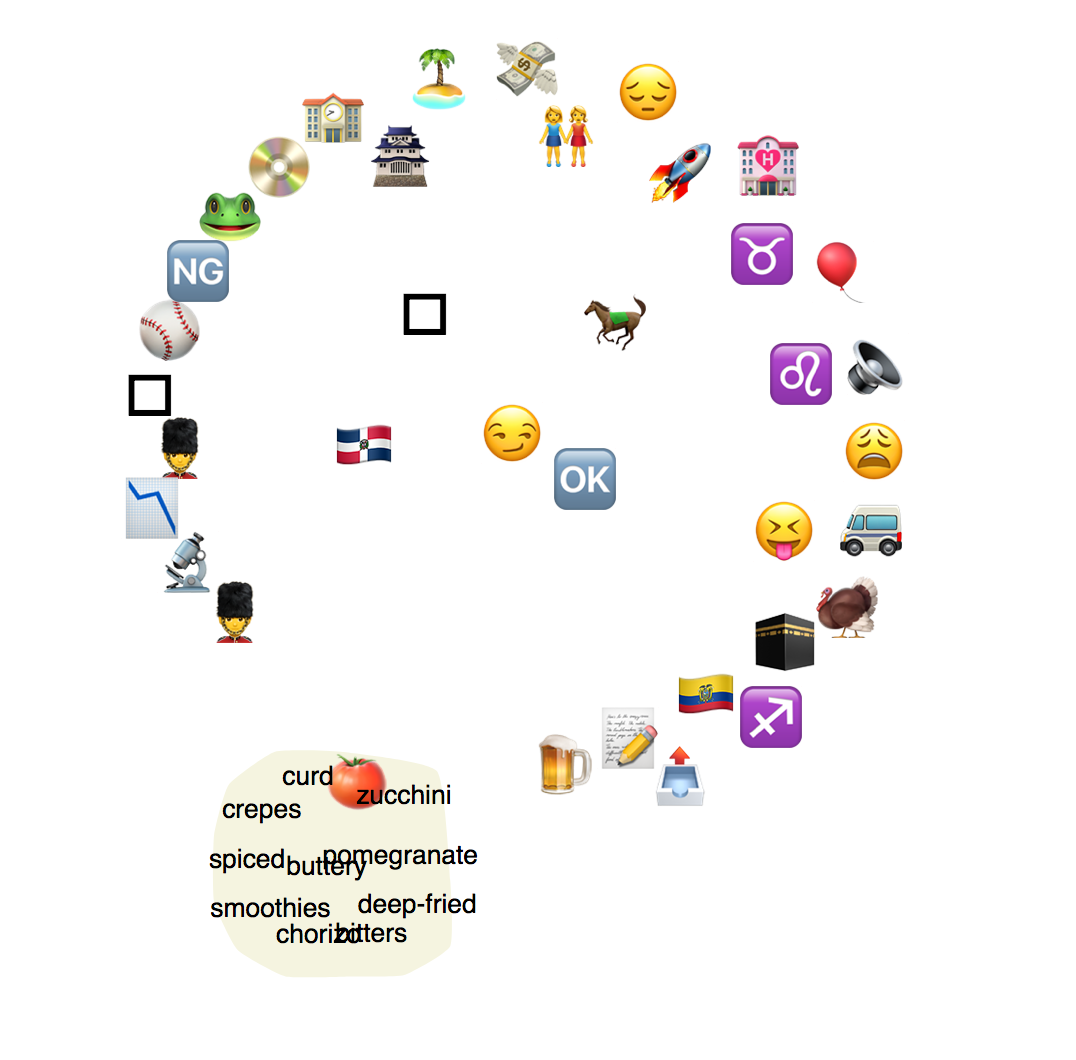
\includegraphics[width=0.68\linewidth]{figures/clustered_network.png}}
    \vspace{-1ex}
     \caption{The visualizaiton of word embeddings using clustered network and emojis.}
\label{fig:cluster_network}
\end{figure}


Our approach for constructing the visualization is as follows:
\begin{enumerate}
 \item Train a word embedding
 \item Run k-means and obtain clusters
 \item Assign an emoji to each cluster
 \item Visualize using D3.js
\end{enumerate}

\subsection{Annotation of Clusters with Emojis}
When a human look at emoji, one connects with various possible concepts. 
Searching for a right word to represent the cluster requires external linguistic resources e.g., WordNet. 
However, images does not associate a single word. 
For example, when one looks at 🍅, the possible association of this words are ``tomato'', ``vegatable'', ``food'', or even ``object''. 
Therefore, we decide to use emojis to represent the clusters. 


\subsection{Interaction}
Users can click on emojis to ``drill-down'' \cite{Elmqvist:2010:HAI:1749404.1749525} the cluster and look into which words are in the cluster.


\subsection{Force Layout}
To solve the problem of overlapping texts, we also use force layout in D3.js to let the texts and emojis move and draggable. 

\section{Discussion}
\label{sec:discussion}

\paragraph{Outliers} 

\paragraph{Emojis are diverse} 

\paragraph{\bf Emojis Captures Approximate Meaning} 
One of the successful cases of our visualization is a cluster with the spacecraft emoji 🚀 annotated. This cluster contains transportation-related words such as ``c-130'' and ``refueling''. 

On the other hand, some emojis (e.g., Leo emoji) are harder to interpret what does a cluster mean. 
Furthermore, one emoji could have multiple descriptions (e.g., the descriptions for the leo emoji are ``greek'', ``sign'', ``zodiac'', ``stars'', ``constellation'', ``astrology'', ``lion'') which further requires sophisticated processing when we want to improve the quality of the visualization. 

\paragraph{\bf We cannot avoid clutters when data points become large ($>5000$)} 
The problem of visual cluttering is still unresolved when the number of data points we want to visualize become large. 
Since we only made the drill available by one level,even assigning 100 words per cluster would cause visualization clutter. 


%\bibliographystyle{abbrv}
\bibliographystyle{abbrv-doi}
%\bibliographystyle{abbrv-doi-narrow}
%\bibliographystyle{abbrv-doi-hyperref}
%\bibliographystyle{abbrv-doi-hyperref-narrow}

\bibliography{template,journal-full,yoshinari}
\end{document}
